\documentclass[aspectratio=169]{beamer}

\useoutertheme{infolines}

\usepackage{graphicx}

\title{PNLSS Identification}
\subtitle{Post Institute Meeting 1}
\author[Balaji, N. N.]{Nidish Narayanaa Balaji}
\institute[Rice U.]{Rice University, Houston, TX 77005}
\date{September 19, 2019}
\begin{document}
\maketitle{}

\begin{frame}
  \frametitle{Overview}
  \begin{itemize}
  \item The main issues we were previously having with the PNLSS
    identification were:
    \begin{enumerate}
    \item \textbf{Forcing levels leading to \underbar{periodic input}
      $\implies$ \underbar{non-periodic response}:} PNLSS was unable to
      identify the model to sufficient error even in the time domain
    \item \textbf{Identification of frictional systems:} Identified models seem
      to perform better only around the \underbar{regime of response} contained
      in the training data
    \item \textbf{Implementation of output-only non-linearities:} Not
      very reliable. Questions:
      \begin{itemize}
      \item Has to be non-hysteretic?
      \item Linearity in coefficients? 
      \item Is this even appropriate for friction non-linearities?
      \end{itemize}
    \end{enumerate}
  \item Currently focused on \underbar{aspect 1}: Investigation of
    non-periodic responses.
  \item The suggestion was to try to increase the damping to reduce
    such a regime.
\end{itemize}
\end{frame}

\begin{frame}[fragile,allowframebreaks]
  \frametitle{Periodic Input - Non-periodic Response}
  \framesubtitle{Training using Data With Transients}
  \begin{columns}
    \begin{column}{0.5\linewidth}
      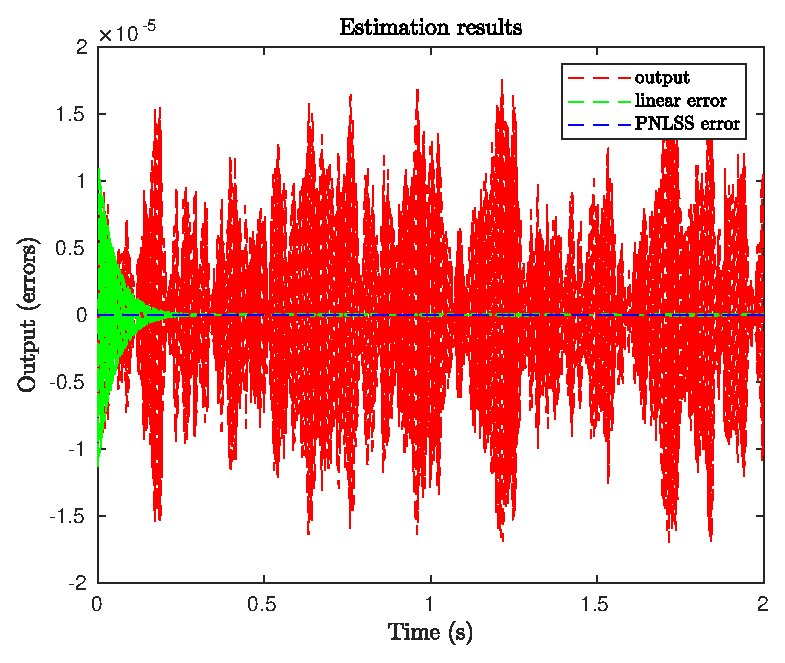
\includegraphics[width=\linewidth]{{{figs/TDOMESTRESS_PNLSS_A0.01_F4096_nx23}}}
    \end{column}%
    \begin{column}{0.5\linewidth}
      \begin{itemize}
      \item Found routine \verb|fLMnlssWeighted_x0u0| which estimates
        initial conditions along with parameters
      \item This could be used to successfully train transient data
        for the Duffing problem (see left)
      \item $n_x = [2, 3]$ used here
      \end{itemize}
    \end{column}
  \end{columns}

  \begin{columns}
    \begin{column}{0.25\linewidth}
      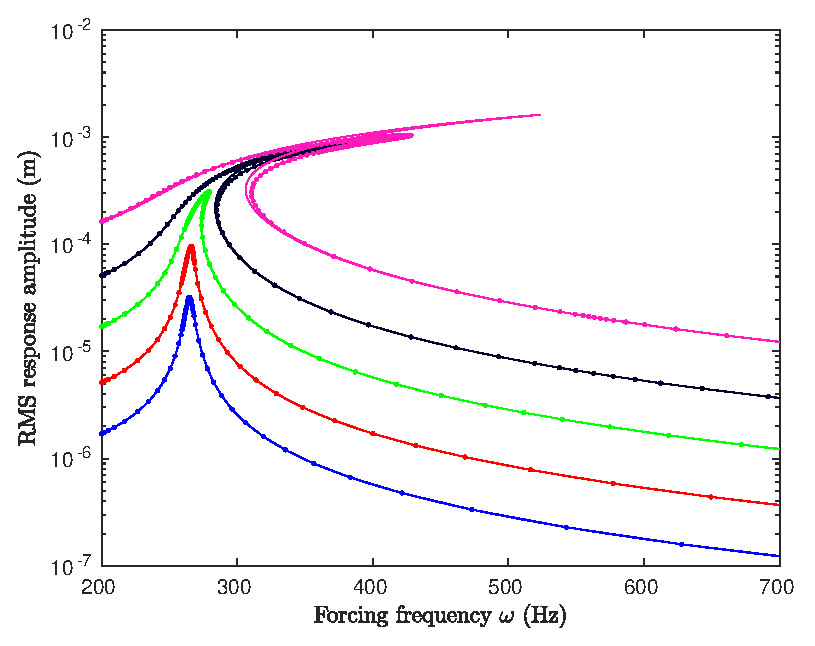
\includegraphics[width=\linewidth]{{{figs/pnlssfrf_A0.01_Amp_nx23}}}
      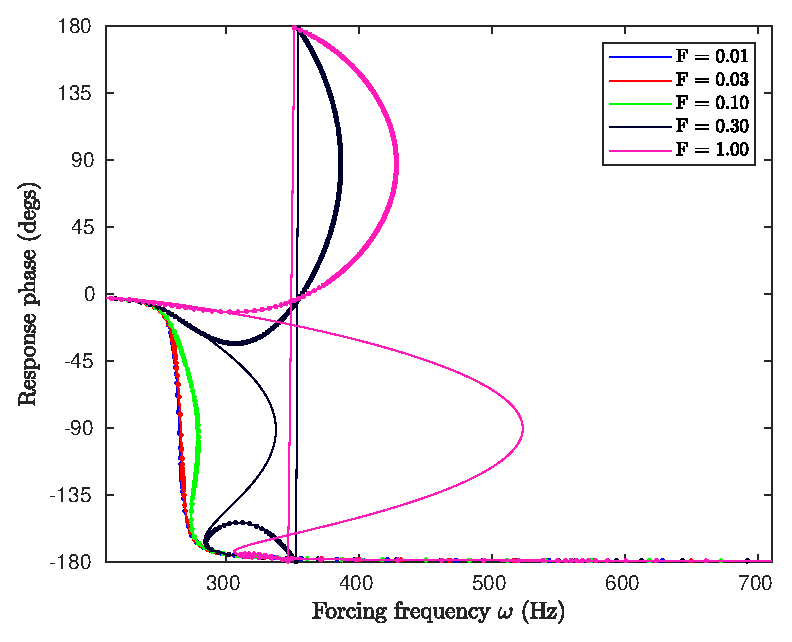
\includegraphics[width=\linewidth]{{{figs/pnlssfrf_A0.01_Phase_nx23}}}

      {\hspace{1cm} A = 0.01}
    \end{column}%
    \begin{column}{0.75\linewidth}
      \begin{itemize}
      \item The data has response with peak amplitude $2\times
        10^{-4}$ m
      \item The identification works fine until the required response
        level on the frequency response diagram is about one magnitude
        higher than this
      \item The damping factor has already been increased
      \end{itemize}
      
      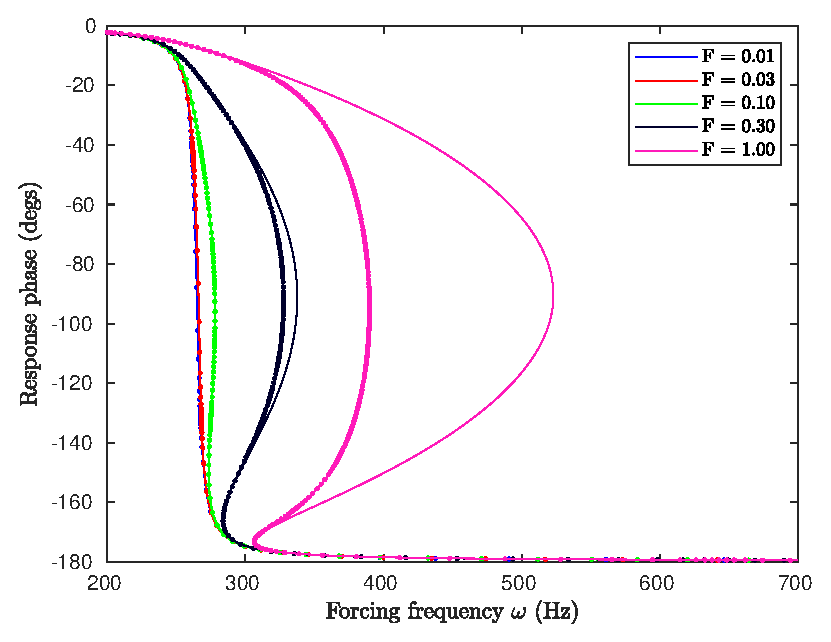
\includegraphics[width=0.333\linewidth]{{{figs/pnlssfrf_A0.25_Phase_nx23}}}%
      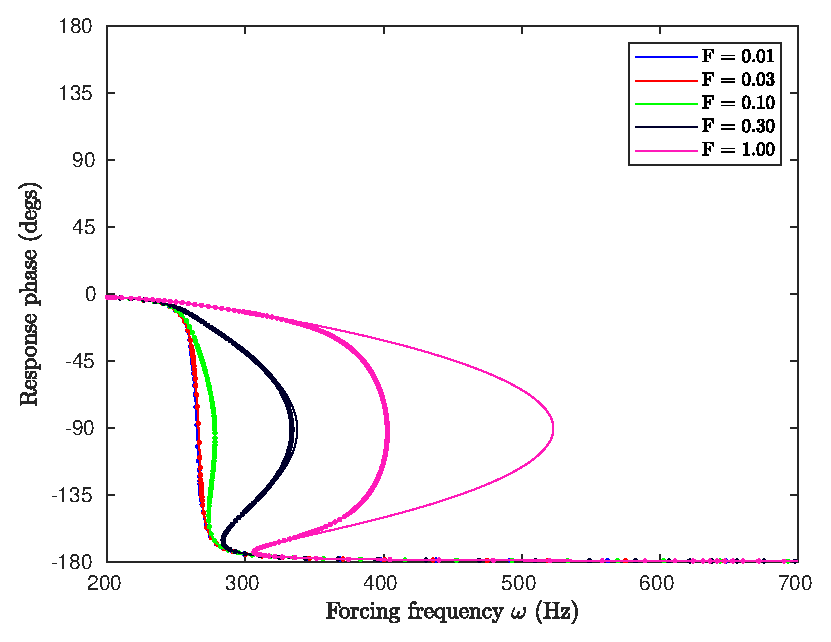
\includegraphics[width=0.333\linewidth]{{{figs/pnlssfrf_A0.50_Phase_nx23}}}%
      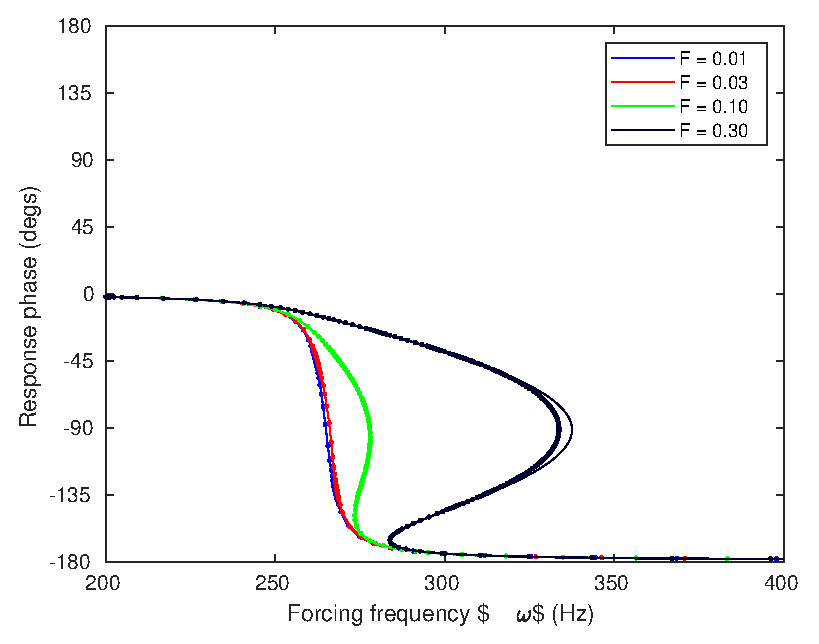
\includegraphics[width=0.333\linewidth]{{{figs/pnlssfrf_A0.75_Phase_nx23}}}

      \hspace{1.5cm}A=0.25
      \hspace{2.5cm}A=0.50
      \hspace{2.5cm}A=0.75
    \end{column}
  \end{columns}
\end{frame}

\begin{frame}
  \frametitle{Periodic Input - Non-periodic Response}
  \begin{columns}
    \begin{column}{0.4\linewidth}
      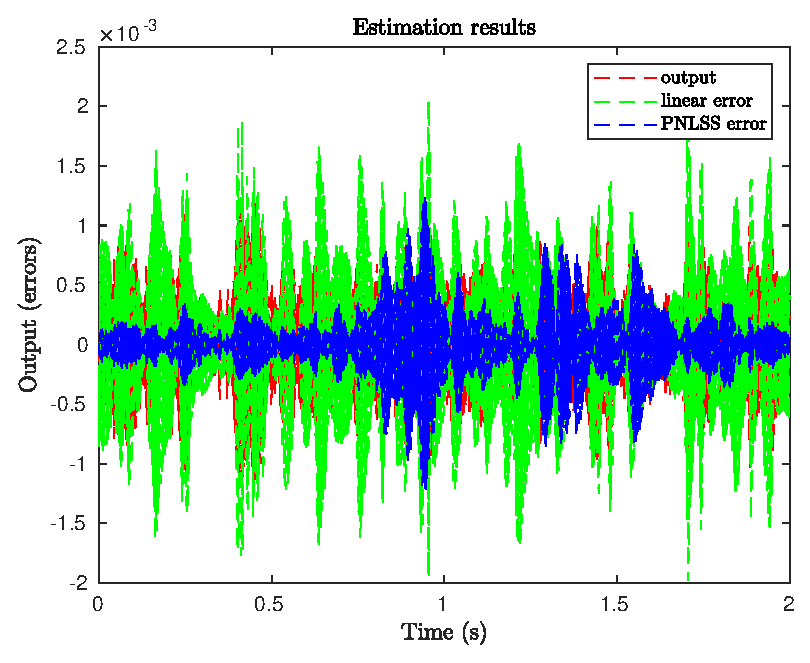
\includegraphics[width=\linewidth]{{{figs/TDOMESTRESS_PNLSS_A0.75_F4096_nx23}}}
      \begin{itemize}
      \item This issue persists even upon increasing the number of
        states to $n_x = [2, 3, 4, 5]$
      \end{itemize}
    \end{column}%
    \begin{column}{0.6\linewidth}
      \begin{itemize}
      \item For the larger amplitude case (when the response seems to
        lose periodicity), PNLSS is unable to perform very well
      \item This is also reflected in the frf's:
      \end{itemize}
      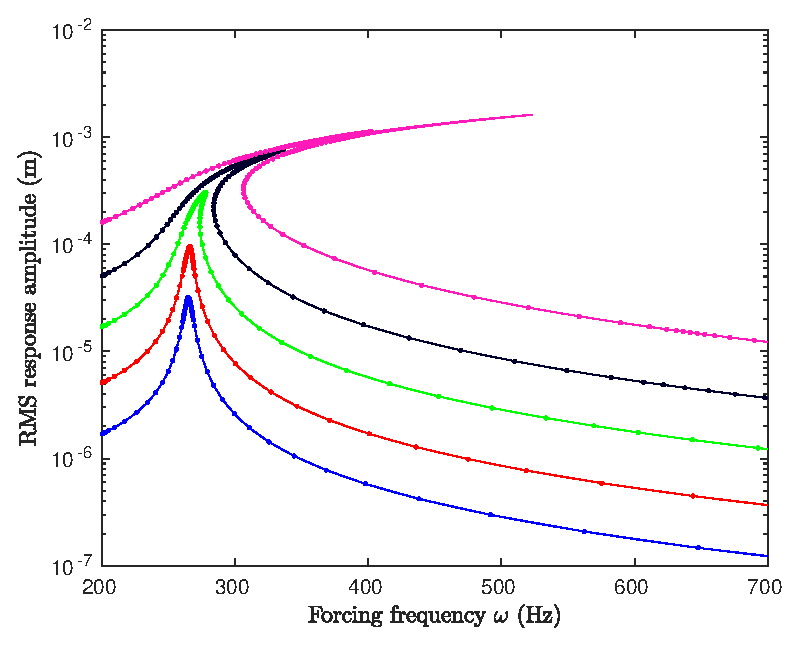
\includegraphics[width=0.5\linewidth]{{{figs/pnlssfrf_A0.50_Amp_nx23}}}%
      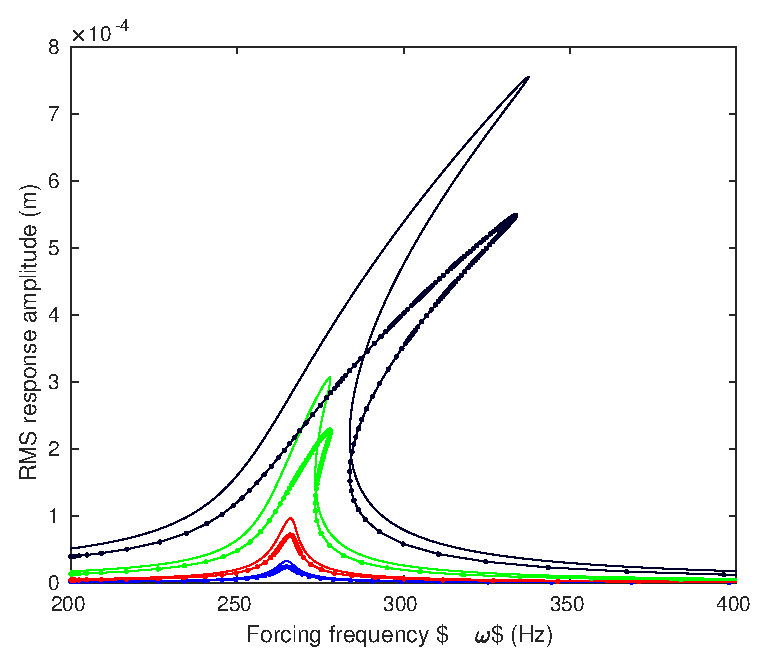
\includegraphics[width=0.5\linewidth]{{{figs/pnlssfrf_A0.75_Amp_nx23}}}
      
      \hspace{1.8cm}A=0.50\hspace{3.25cm}A=0.75
    \end{column}
  \end{columns}
\end{frame}

\end{document}
%%% Local Variables:
%%% mode: latex
%%% TeX-master: t
%%% End:
